%!TEX root = ../thesis.tex

\cleardoublepage
\chapter{Evaluation}
\label{cha:evaluation}

This chapter reviews how the approach from the previous chapter was tested, and it discusses the observed results. The goal here is to explain the setup of the testbed, as well as the motivation behind the types of tests which were performed. Finally a discussion of the results and their implications will take place.


\section{Approach to Evaluating Performance}

In order to evaluate the success of the proposed approach, multipath scenarios will be emulated and investigated. Each setup will consist of two WAN connectors, and some number of emulated links going between them. Due to the expectation that satellite backhaul will become more and more relevant for geographically distributed campus networks, the emulation will feature a Low Earth Orbit (LEO) satelltile link as well as a Geostationsary Orbit (GEO) link, and a terrestrial connection, which will be based on the characteristics of DSL or perhaps earlier DOCSIS links, but specifically \textbf{not} optical fibre. This thesis is addressed towards campus network deployments that do not have access to fibre yet, and cannot expect to receive it in the near future.

\begin{figure}[h]
    \centering
        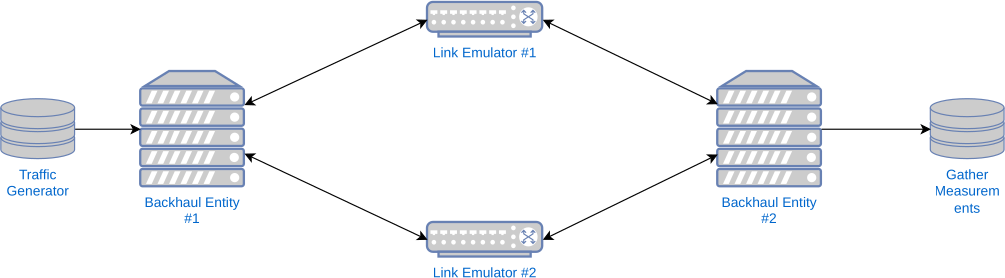
\includegraphics[width=0.66\textwidth]{fig/testbed.png}
        \caption{Testbed Setup}
        \label{fig:testbed}
\end{figure}

In all of these scenarios the same traffic flows will be replayed. This traffic will contain different types of flows, with different QoS requirements. Before a new flow is started, the flow's requirements are sent to the WAN connector and it is either accepted or rejected. During the traffic replay, the delay, jitter, and reliability will be measured.

All of these tests can be performed on the same testbed which will be set up as is shown in Figure \ref{fig:testbed}. The testbed architecture features a traffic generator, two WAN connectors, with a link emulator between them, and a measurement module to analyze performance. In practice the traffic generator and the test bench will be co-located on the same machine. The link emulator, and the WAN connectors are separate hosts, all interconnected over ethernet. The link emulation is done using the linux kernel's traffic control subsytem (TC). TC offers a network emulator (netem) queuing discipline (qdisc), which is able to emulate various link characteristics including delay, jitter, packet loss and packet re-ordering. Furthermore by combining the netem qdisc with a rate limiter, such as the Heirarchical Token Bucket (HTB) qdisc, a link can have its bandwidth limited. This allows one to emulate links with different latency, reliability and jitter, and with different maximum bandwidths.

In order to make the emulation more realistic, it will periodically be adjusted, this allows one to degrade a link over time, for example by increasing the latency or packet loss in frequent intervals, up to a large value. It also more closely mimics the real-life behavior of WAN connections, which do experience changes in their characteristics over time.

For the purposes of evaluating the WAN connector, two initial series of experiments will be performed to isolate and investigate it's link switching capabilities. Firstly, purely latency based link selection will be investigated- a flow will be defined with specific latency requirements and then the emulated links will have their latency repeatedly changed so that one or more of them begin to violate the maximum latency. The WAN connector should then switch the flow to a different path. The same will be done once with packet loss. First, a  link will be given a packet loss that is higher than the acceptable level for the given flow. Then multiple links will be adjusted so that their level of packet loss is too high to support a flow on its own, later complete link failure will be simulated. This simulation will be done by using the linux packet filtering tool iptables to block all traffic with the source IP of one of the links. These two experiments will both be conducted with other variables held to a control value. So first only the latency will be varied, then only the packet loss. In the expriments with packet loss the WAN connector should at first switch the flow to a different connection, and then later being to duplicate the flow. During the duplication experiment, the application behind the flow should not receive any duplicate packets.

Lastly after the two control experiments have confirmed (or not confirmed) the expected behaviour, a proper test will take place where the links' characteristics are varied independently of each other and once again a select few critical flows will be observed, to make sure the WAN connector is able to uphold their QoS requirements.


\section{Latency Based Path Switching}
\section{Reliability Based Path Switching}

\section{Extended Experiments}